%%
%% Beginning of file 'sample.tex'
%%
%% Modified 2015 December
%%
%% This is a sample manuscript marked up using the
%% AASTeX v6.x LaTeX 2e macros.

%% AASTeX is now based on Alexey Vikhlinin's emulateapj.cls 
%% (Copyright 2000-2015).  See the classfile for details.
%%
%% AASTeX requires revtex4-1.cls (http://publish.aps.org/revtex4/) and
%% other external packages (latexsym, graphicx, amssymb, longtable, and epsf).
%% All of these external packages should already be present in the modern TeX 
%% distributions.  If not they can also be obtained at www.ctan.org.

%% The first piece of markup in an AASTeX v6.x document is the \documentclass
%% command. LaTeX will ignore any data that comes before this command. The 
%% documentclass can take an optional argument to modify the output style.
%% The command below calls the preprint style  which will produce a tightly 
%% typeset, one-column, single-spaced document.  It is the default and thus
%% does not need to be explicitly stated.
%%

%% using aastex version 6
\documentclass[onecolumn]{aastex6}
\usepackage{subfigure}
\usepackage{amsmath}

%% The other main article choice is a tightly typeset, two-column article
%% that more closely resembles the final typeset pdf article.
%%
%% \documentclass[twocolumn]{aastex6}
%% 
%% There are other optional arguments one can envoke to allow other 
%% actions. 
%%
% These are the available options:
%   manuscript	: onecolumn, doublespace, 12pt fonts
%   preprint	: onecolumn, single space, 10pt fonts
%   preprint2	: twocolumn, single space, 10pt fonts
%   twocolumn	: a two column article. Probably not needed, but here just in case.
%   onecolumn	: a one column article; default option.
%   twocolappendix: make 2 column appendix
%   onecolappendix: make 1 column appendix is the default. 
%   astrosymb	: Loads Astrosymb font and define \astrocommands. 
%   tighten	: Makes baselineskip slightly smaller
%   times	: uses times font instead of the default
%   linenumbers	: turn on lineno package.
%   trackchanges : required to see the revision mark up and print output
%   numberedappendix: Labels appendix sections A, B, ... This is the default.
%   appendixfloats: Needed. Resets figure and table counters to zero

%% these can be used in any combination, e.g.
%%
%% \documentclass[twocolumn,twocolappendix,linenumbers,trackchanges]{aastex6}

%% If you want to create your own macros, you can do so
%% using \newcommand. Your macros should appear before
%% the \begin{document} command.
%%
\newcommand{\vdag}{(v)^\dagger}
\newcommand\aastex{AAS\TeX}
\newcommand\latex{La\TeX}

%% AASTeX 6.0 supports the ability to suppress the names and affiliations
%% of some authors and displaying them under a "collaboration" banner to
%% minimize the amount of author information that to be printed.  This 
%% should be reserved for articles with an extreme number of authors.
%%
%% Mark up commands to limit the number of authors on the front page.
\AuthorCallLimit=2
%% Will only show Schwarz & Muench since Schwarz and Muench
%% are in the same \author call. 
\fullcollaborationName{The Friends of AASTeX Collaboration}
%% will print the collaboration text after the shortened author list.
%% These commands have to COME BEFORE the \author calls.
%%
%% Note that all of these author will be shown in the published article.
%% This feature is meant to be used prior to acceptance to make the
%% front end of a long author article more manageable.
%% Use \allauthors at the manuscript end to show the full author list.

%% The following command can be used to set the latex table counters.  It
%% is needed in this document because it uses a mix of latex tabular and
%% AASTeX deluxetables.  In general it should not be needed.
%\setcounter{table}{1}

%%%%%%%%%%%%%%%%%%%%%%%%%%%%%%%%%%%%%%%%%%%%%%%%%%%%%%%%%%%%%%%%%%%%%%%%%%%%%%%%
%%
%% The following commented section outlines numerous optional output that
%% can be displayed in the front matter or as running meta-data.
%%
%% You can insert a short comment on the title page using the command below.
%% \slugcomment{Not to appear in Nonlearned J., 45.}
%%
%% If you wish, you may supply running head information, although
%% this information may be modified by the editorial offices.
%%\shorttitle{\aastex sample article}
%%\shortauthors{Schwarz et al.}
%%
%% You can add a light gray and diagonal water-mark to the first page 
%% with this command:
%% \watermark{text}
%% where "text", e.g. DRAFT, is the text to appear.  If the text is 
%% long you can control the water-mark size with:
%% \setwatermarkfontsize{dimension}
%% where dimension is any recognized LaTeX dimension, e.g. pt, in, etc.
%%
%%%%%%%%%%%%%%%%%%%%%%%%%%%%%%%%%%%%%%%%%%%%%%%%%%%%%%%%%%%%%%%%%%%%%%%%%%%%%%%%

%% This is the end of the preamble.  Indicate the beginning of the
%% paper itself with \begin{document}.

\begin{document}

%% LaTeX will automatically break titles if they run longer than
%% one line. However, you may use \\ to force a line break if
%% you desire.

\title{HW 01: The Distance to the Pleiades}

%% Use \author, \affil, plus the \and command to format author and affiliation 
%% information.  If done correctly the peer review system will be able to
%% automatically put the author and affiliation information from the manuscript
%% and save the corresponding author the trouble of entering it by hand.
%%
%% The \affil should be used to document primary affiliations and the
%% \altaffil should be used for secondary affiliations, titles, or email.

%% Authors with the same affiliation can be grouped in a single
%% \author and \affil call.
\author{Bryan Yamashiro\altaffilmark{1}}
\affil{University of Hawaii at Manoa \\
2500 Campus Road \\
Honolulu, HI 96822}


%% Use the \and command so offset the last author.

%% Notice that each of these authors has alternate affiliations, which
%% are identified by the \altaffilmark after each name.  Specify alternate
%% affiliation information with \altaffiltext, with one command per each
%% affiliation.

%\altaffiltext{1}{A cool dude}
%\altaffiltext{2}{Another cool dude}


%% From the front matter, we move on to the body of the paper.
%% Sections are demarcated by \section and \subsection, respectively.
%% Observe the use of the LaTeX \label
%% command after the \subsection to give a symbolic KEY to the
%% subsection for cross-referencing in a \ref command.
%% You can use LaTeX's \ref and \label commands to keep track of
%% cross-references to sections, equations, tables, and figures.
%% That way, if you change the order of any elements, LaTeX will
%% automatically renumber them.

%% We recommend that authors also use the natbib \citep
%% and \citet commands to identify citations.  The citations are
%% tied to the reference list via symbolic KEYs. The KEY corresponds
%% to the KEY in the \bibitem in the reference list below. 



\section{Introduction}

The parallaxes of the Pleiades galaxy cluster utilizing the HIPPARCOS catalog\,(H-cat) were determined from an angular radius 2$^\circ$ angle of the RA/Dec coordinates, 03h47m00.0s +24d03m00.0s. H-cat was conceived from four years of data collected by the Hipparcos satellite in geostationary orbit\,(\cite{1}). The objective of this study will be to derive a distance to the Pleiades cluster while invoking the various parameters measured by Hipparcos and an arsenal of astrophysical equations.


\section{Observations}

\subsection{Cluster Distance}
There was a total of 57 objects from H-cat, but 11 were rejected due to a large deviation off of the common parallax. The rejected individual objects included lengths that exceeded a 0.5$\sigma$ statistical error above the most common parralax of 8\,mas, shown in figure\,\ref{Parallaxes}. The full list of objects and the subsequently removed outliers are provided in table\,\ref{alldata}.

\begin{figure*}[ht]
  \centering
  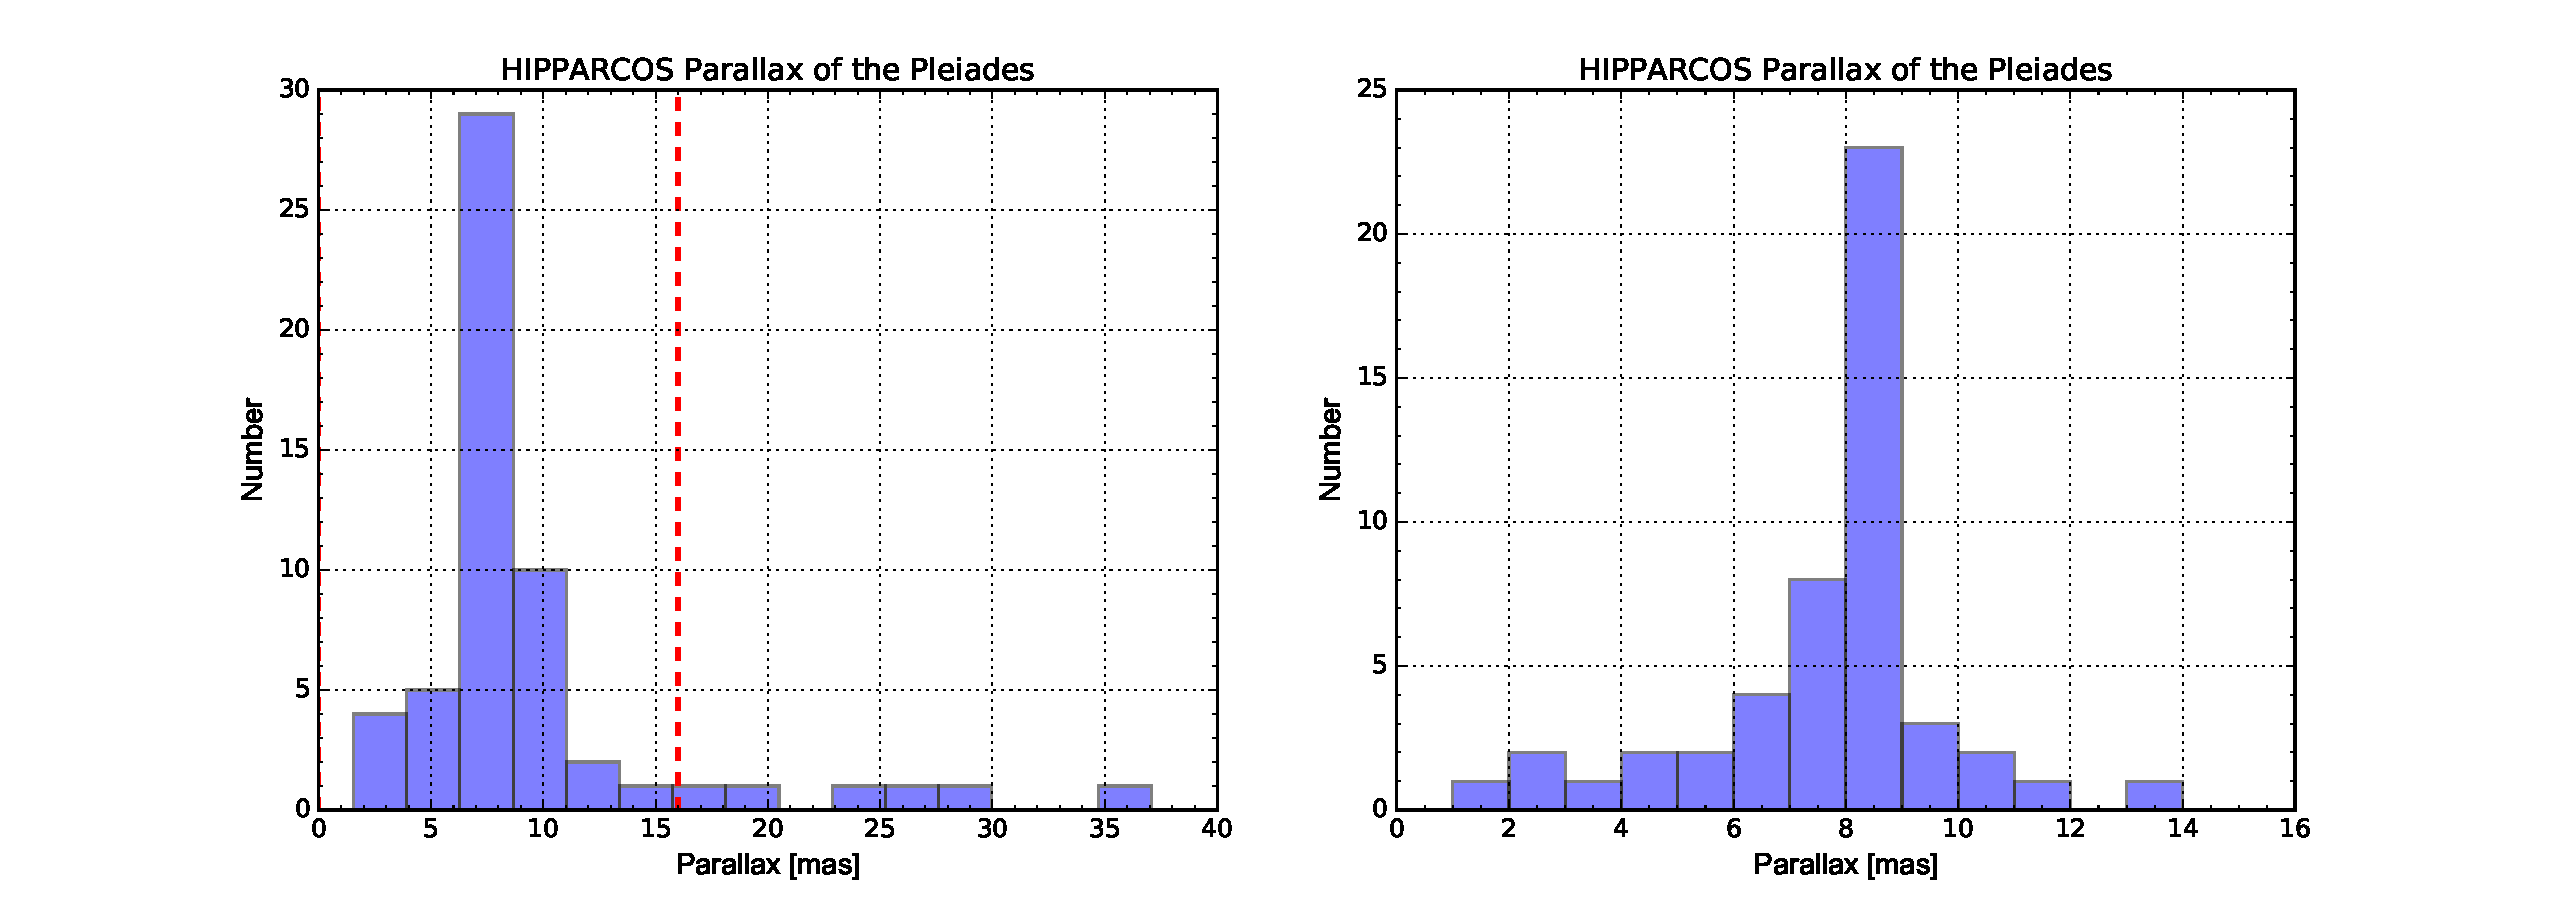
\includegraphics[scale=0.4]{parallax(1).pdf}%\quad
  \caption{The photometric apertures containing both J-star\,(left) and J-standard\,(right). The contour levels are provided to observe the aperture localized intensities of both stars.}
  \label{Parallaxes}
\end{figure*}

The cluster distance was derived using the relationship between an object and the correlating parallax angle, shown in equation\,\ref{dist}\,(\cite{2}). An average of the object distances yielded a distance of (128.5$\pm$15.1)\,pc, within the 2$^\circ$ limit as well as the parallax rejections. The error on the distance was found using error propagation on the parallax and amounted to an average, shown in equation\,\ref{error}.

\begin{equation}
\frac{1}{N}\sum_{i=1}^N \delta x_i
\label{error}
\end{equation}

\begin{equation}
\textnormal{Distance} = \frac{1}{\textnormal{Parallax}}
\label{dist}
\end{equation}

Further testing of the cluster involved the use of the proper motion\,($\mu$), associated with the cluster. H-cat reports $\mu$ in terms of components in RA and Dec, therefore the magnitude is equated from equation\,\ref{propermotion}.

\begin{equation}
\mu = \sqrt{\mu_{RA}^2 + \mu_{Dec}^2}
\label{propermotion}
\end{equation}

Since the proper motions and the distances of each object is defined, the transverse velocity\,(V$_T$) is obtainable. The transverse velocity will not allow for viewing redshift, but it yields an important relation relative to the other bodies. The transverse velocity is obtained via the bodies in motion and their distance, therefore it is implied that objects belonging to the same cluster will yield a linear property with respect to these variables. This linear trait is seen in figure\,\ref{distancevel}\,(right), and promulgates the fact that the rejected objects were indeed not part of the Pleiades. Another method of the object belonging to the cluster was to observe the magnitudes. The two magnitudes parsed included the Hipparcos magnitude\,(Median magnitude in the Hipparcos photometric system), and the (B-V) color index. Again this result showed the deviation that the non-members exhibited and are presented in figure\,\ref{distancevel}\,(left).

\begin{equation}
V_T = \mu D
\end{equation}

\begin{figure*}[ht]
  \centering
  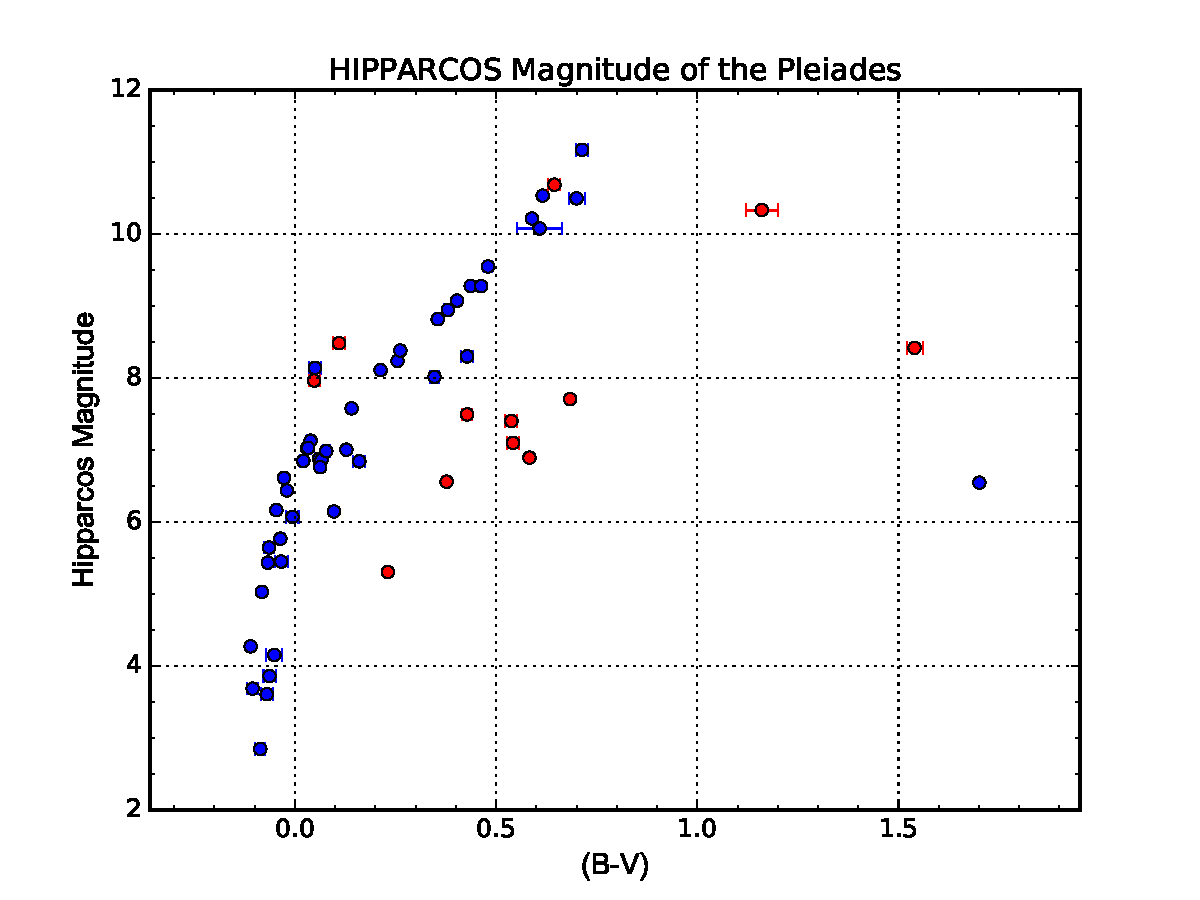
\includegraphics[scale=0.4]{magnitude.pdf}%\quad
  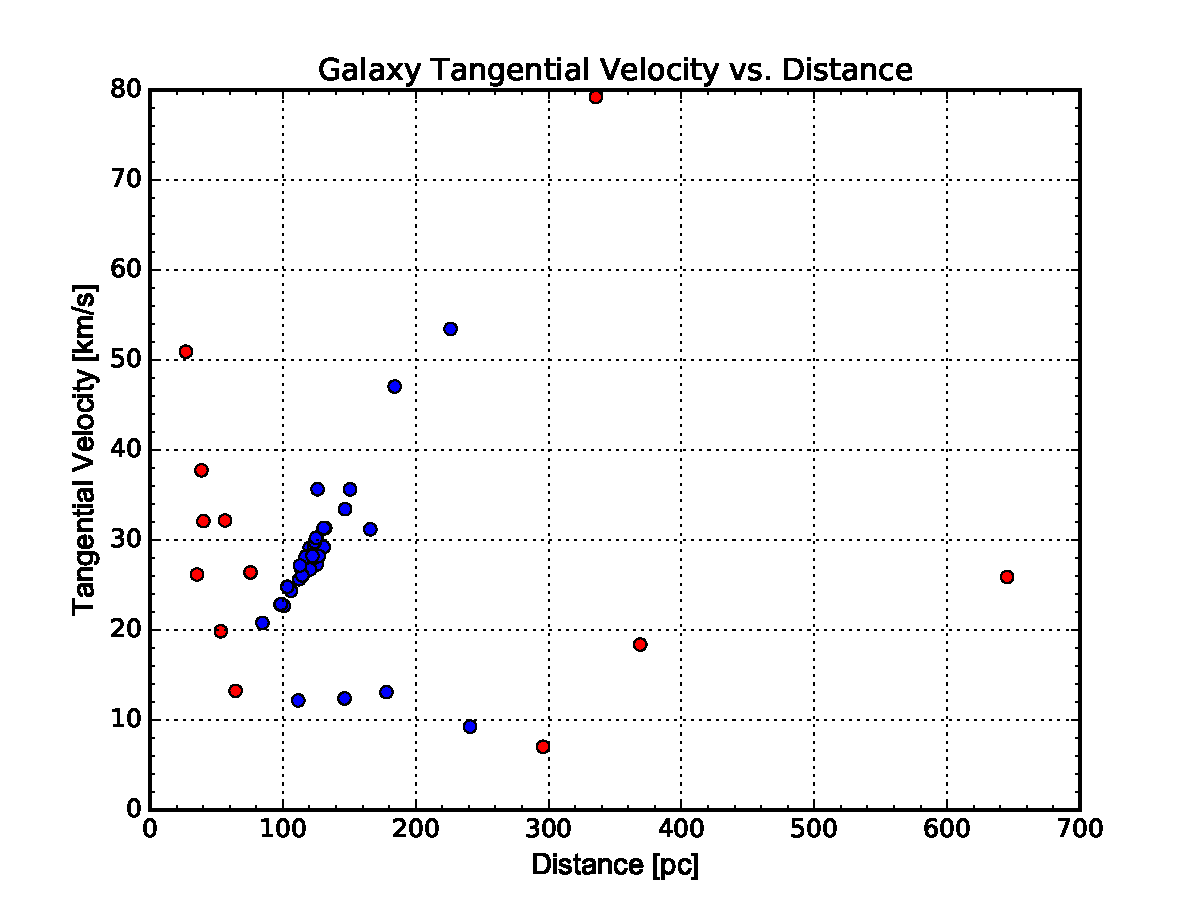
\includegraphics[scale=0.4]{distancevel.pdf}%\quad

  \caption{\textbf{Left: } The color magnitude against the Hipparcos magnitude. The points in red represent the rejected objects, and the magnitudes are clearly not part of the spectrum. \textbf{Right: } The calculated distances against the derived tangential velocities. Red points represent rejected objects, and these show a clear deviation from the main cluster, which is somewhat linear as expected.}
  \label{distancevel}
\end{figure*}



\subsection{Size of the Pleiades}

The general size of the Pleiades for a distance of (128.5$\pm$15.1)\,pc and a 2$^\circ$ angular radius was found with trigonometry in equation\,\ref{trig}. The cluster size was found to be (201.8$\pm$23.7)\,pc across. This size is assuming that the cluster is symmetric and does not extrude variably in the direction toward and away from the viewer.

\begin{equation}
2\times (128.5\textnormal{pc}\pm15.1\textnormal{pc}) \times \arctan{(1^{\circ})} = \textnormal{Cluster Size}
\label{trig}
\end{equation}

\section{Conclusion}

The distance to the Pleiades cluster, utilizing the Hipparcos database, was (128.5$\pm$15.1)\,pc for a 2$^\circ$ angular radius. Subsequently, the cluster size was (201.8$\pm$23.7)\,pc across the perpendicular plane of the sky. The Hipparcos team measured the Pleiades distance at 120.2\,pc\,(\cite{3}), which is within the error of the calculated distance of this study. Against the Hipparcos study, the result obtained in this study yielded a sigma deviation of 0.55$\sigma$.




%---------Procedure Notes

\clearpage
\section{Results}

\begin{deluxetable}{cccccccccc}
\tablecaption{Apparent Magnitude Data \label{tab:mathmode}}
\tablecolumns{10}
\tablenum{1}
\tablewidth{0pt}
\tablehead{
\colhead{Object} & \colhead{RA} & \colhead{Dec}  & \colhead{Parallax }& \colhead{Distance to } & \colhead{Proper Motion } & \colhead{Proper Motion } & \colhead{Magnitude}& \colhead{B-V} \\
\colhead{Number} & \colhead{[deg]} & \colhead{[deg]} & \colhead{[mas]}&  \colhead{Galaxy [pc]} & \colhead{ RA[mas/yr]} & \colhead{Dec [mas/yr]} & \colhead{ [mag]}& \colhead{[mag]} }
\centering
\startdata
16996 & 54.649 & 24.601 & 8.96  $\pm$1.07  &111.607$\pm$13.3           & 3.47    $\pm$1.55  &-22.69  $\pm$1.46    &8.300 $\pm$0.0012  &0.428   $\pm$0.015 \\
17020* & 54.736 & 24.569 & 2.98  $\pm$2.75 &335.570           & 21.24   $\pm$3.71  &-44.93  $\pm$3.32    &10.68 $\pm$0.0041  &0.645   $\pm$0.015 \\
17034 & 54.777 & 24.702 & 8.32  $\pm$0.79  &120.192$\pm$11.4         & 23.91   $\pm$0.97  &-45.11  $\pm$0.74    &7.128 $\pm$0.0008  &0.039   $\pm$0.008 \\
17044 & 54.806 & 24.466 & 10.19 $\pm$2.19  &98.1354$\pm$7.6            & 23.24   $\pm$2.62  &-43.11  $\pm$2.16    &10.53 $\pm$0.004   &0.616   $\pm$0.005 \\
17091 & 54.921 & 23.290 & 11.82 $\pm$1.94  &84.6023$\pm$15.7           & 26.82   $\pm$2.74  &-44.23  $\pm$2.11    &10.07 $\pm$0.005   &0.608   $\pm$0.056 \\
17181 & 55.192 & 25.329 & 6.83  $\pm$0.5   &146.412$\pm$41.6         & 9.83    $\pm$0.58  &-14.86  $\pm$0.5     &6.146 $\pm$0.0009  &0.097   $\pm$0.005 \\
17225 & 55.345 & 23.487 & 8.1   $\pm$1.06  &123.456$\pm$7.6          & 21.78   $\pm$1.42  &-44.97  $\pm$1.26    &9.279 $\pm$0.0019  &0.437   $\pm$0.006 \\
17245 & 55.400 & 25.619 & 6.64  $\pm$1.51  &150.602$\pm$24             & 14.67   $\pm$1.8   &-47.59  $\pm$1.67    &10.21 $\pm$0.0026  &0.589   $\pm$0.004 \\
17289 & 55.519 & 22.858 & 7.65  $\pm$1.5   &130.718$\pm$25.8           & 20.04   $\pm$1.89  &-42.56  $\pm$1.51    &9.274 $\pm$0.0024  &0.463   $\pm$0.003 \\
17305* & 55.566 & 22.786 & 18.77 $\pm$0.84 &53.2765         & 20.81   $\pm$1.03  &-75.66  $\pm$0.88    &7.494 $\pm$0.0009  &0.428   $\pm$0.013 \\
17317 & 55.600 & 22.421 & 8.27  $\pm$2.07  &120.918$\pm$21.9           & 18.87   $\pm$2.22  &-43.38  $\pm$1.71    &10.49 $\pm$0.0051  &0.7     $\pm$0.02 \\
17401 & 55.923 & 23.649 & 7.58  $\pm$0.9   &131.926$\pm$36         & 18.77   $\pm$1.06  &-46.36  $\pm$0.95    &8.016 $\pm$0.0013  &0.347   $\pm$0.01 \\
17403 & 55.929 & 25.080 & 7.93  $\pm$0.6   &126.103$\pm$14.3         & 22.38   $\pm$0.97  &-55.13  $\pm$0.98    &7.577 $\pm$0.0015  &0.141   $\pm$0.008 \\
17489 & 56.200 & 24.289 & 8.65  $\pm$0.36  &115.606$\pm$8              & 20.38   $\pm$0.43  &-44.81  $\pm$0.37    &5.450 $\pm$0.0006  &-0.034  $\pm$0.016 \\
17497 & 56.213 & 23.269 & 8.33  $\pm$1.22  &120.048$\pm$5.2          & 21.87   $\pm$1.37  &-43.18  $\pm$1.08    &9.074 $\pm$0.0019  &0.403   $\pm$0.007 \\
17499 & 56.218 & 24.113 & 8.06  $\pm$0.25  &124.069$\pm$18.8         & 20.84   $\pm$0.28  &-46.06  $\pm$0.23    &3.685 $\pm$0.0006  &-0.105  $\pm$0.013 \\
17527 & 56.290 & 24.839 & 7.97  $\pm$0.37  &125.470$\pm$3.9          & 20.36   $\pm$0.45  &-46.52  $\pm$0.41    &5.644 $\pm$0.0006  &-0.064  $\pm$0.012 \\
17531 & 56.302 & 24.467 & 7.97  $\pm$0.33  &125.470$\pm$5.8            & 21.24   $\pm$0.38  &-40.56  $\pm$0.35    &4.272 $\pm$0.0006  &-0.11   $\pm$0.006 \\
17572 & 56.453 & 23.147 & 8.24  $\pm$0.75  &121.359$\pm$4.9          & 20.5    $\pm$0.85  &-44.55  $\pm$0.74    &6.875 $\pm$0.0011  &0.06    $\pm$0.011 \\
17573 & 56.456 & 24.367 & 8.51  $\pm$0.28  &117.508$\pm$10.4         & 20.95   $\pm$0.31  &-45.98  $\pm$0.28    &3.859 $\pm$0.0006  &-0.063  $\pm$0.015 \\
17579 & 56.476 & 24.554 & 8.77  $\pm$0.54  &114.025$\pm$3.6            & 20.18   $\pm$0.7   &-44.87  $\pm$0.62    &5.767 $\pm$0.0011  &-0.036  $\pm$0.008 \\
17583 & 56.496 & 25.398 & 8     $\pm$0.89  &125    $\pm$8.4          & 19      $\pm$0.99  & -47.23 $\pm$0.94    &8.108 $\pm$0.0012  &0.213   $\pm$0.006 \\
17588 & 56.512 & 24.528 & 8.58  $\pm$0.56  &116.550$\pm$12.1           & 19.88   $\pm$0.73  &-44.37  $\pm$0.65    &6.438 $\pm$0.0012  &-0.02   $\pm$0.006 \\
17608 & 56.581 & 23.948 & 8.58  $\pm$0.37  &116.550$\pm$7.6            & 21.13   $\pm$0.35  &-43.65  $\pm$0.27    &4.153 $\pm$0.001   &-0.051  $\pm$0.02 \\
17625 & 56.645 & 25.843 & 4.42  $\pm$1.48  &226.244$\pm$18.9         & 20.91   $\pm$1.65  &-45.13  $\pm$1.38    &8.816 $\pm$0.002   &0.355   $\pm$0.007 \\
17664 & 56.747 & 24.520 & 7.66  $\pm$0.66  &130.548$\pm$25.2           & 22.73   $\pm$0.84  &-45     $\pm$0.85    &6.848 $\pm$0.0006  &0.021   $\pm$0.007 \\
17684* & 56.821 & 23.726 & 15.52 $\pm$0.73 &64.4329           & -34.94  $\pm$0.69  &-25.54  $\pm$0.55    &7.098 $\pm$0.0017  &0.542   $\pm$0.014 \\
17692 & 56.837 & 23.803 & 8.9   $\pm$0.77  &112.359$\pm$8.3          & 18.56   $\pm$0.75  &-44.31  $\pm$0.6     &7.022 $\pm$0.0011  &0.03    $\pm$0.001 \\
17694 & 56.845 & 22.922 & 8.62  $\pm$0.84  &116.009$\pm$10.4       & 20.91   $\pm$1.04  &-44.88  $\pm$0.87    &8.238 $\pm$0.0012  &0.255   $\pm$0.004 \\
17702 & 56.871 & 24.105 & 8.09  $\pm$0.42  &123.609$\pm$12.8           & 19.34   $\pm$0.39  &-43.67  $\pm$0.33    &2.848 $\pm$0.0006  &-0.086  $\pm$0.012 \\
17704 & 56.872 & 24.288 & 9.42  $\pm$0.75  &106.157$\pm$4.7          & 18.33   $\pm$0.87  &-44.69  $\pm$0.74    &6.859 $\pm$0.0013  &0.066   $\pm$0.006 \\
17729 & 56.945 & 25.385 & 9.68  $\pm$0.93  &103.305$\pm$8              & 19.26   $\pm$0.96  &-46.75  $\pm$0.91    &8.381 $\pm$0.001   &0.262   $\pm$0.008 \\
17759 & 57.027 & 24.988 & 6.03  $\pm$0.7   &165.837$\pm$25.6           & -28     $\pm$0.78  &-28     $\pm$0.74    &6.546 $\pm$0.0044  &1.701   $\pm$0.001 \\
17776 & 57.086 & 23.421 & 8.45  $\pm$0.39  &118.343$\pm$9.8            & 17.99   $\pm$0.39  &-46.57  $\pm$0.32    &5.435 $\pm$0.0008  &-0.067  $\pm$0.008 \\
17791 & 57.125 & 24.345 & 7.87  $\pm$1.32  &127.064$\pm$21.3         & 17.68   $\pm$1.48  &-43.28  $\pm$1.37    &7.003 $\pm$0.0013  &0.128   $\pm$0.005 \\
17812* & 57.174 & 25.800 & 3.38  $\pm$1.06 &295.857         & -2.22   $\pm$1.53  &-4.48   $\pm$1.74    &8.482 $\pm$0.0023  &0.11    $\pm$0.015 \\
17828 & 57.227 & 22.799 & 4.15  $\pm$0.97  &240.963$\pm$56.3         & 6.76    $\pm$1.14  &-4.45   $\pm$0.93    &8.139 $\pm$0.0027  &0.05    $\pm$0.015 \\
17832* & 57.237 & 23.857 & 13.22 $\pm$0.52  &75.6429         & 46.63   $\pm$0.53  &-56.75  $\pm$0.44    &6.559 $\pm$0.0008  &0.377   $\pm$0.009 \\
17847 & 57.290 & 24.053 & 8.53  $\pm$0.39  &117.233$\pm$13.3          & 17.7    $\pm$0.36  &-44.18  $\pm$0.32    &3.608 $\pm$0.001   &-0.07   $\pm$0.015 \\
17851 & 57.296 & 24.136 & 8.54  $\pm$0.31  &117.096$\pm$5.3          & 18.07   $\pm$0.3   &-47.2   $\pm$0.27    &5.029 $\pm$0.0017  &-0.082  $\pm$0.004 \\
17862 & 57.340 & 24.381 & 8.18  $\pm$0.59  &122.249$\pm$4.6          & 17.42   $\pm$0.65  &-45.38  $\pm$0.52    &6.611 $\pm$0.0012  &-0.027  $\pm$0.004 \\
17892 & 57.409 & 22.533 & 8.3   $\pm$0.66  &120.481$\pm$8.6            & 18.52   $\pm$0.8   &-42.87  $\pm$0.65    &7.030 $\pm$0.0011  &0.033   $\pm$0.008 \\
17900 & 57.431 & 23.711 & 8.72  $\pm$0.6   &114.678$\pm$8.7          & 16.73   $\pm$0.63  &-44.82  $\pm$0.53    &6.164 $\pm$0.0009  &-0.046  $\pm$0.007 \\
17921 & 57.479 & 22.244 & 8.86  $\pm$0.42  &112.866$\pm$7.6             & 24.31   $\pm$0.48  &-44.46  $\pm$0.39    &6.072 $\pm$0.0006  &-0.006  $\pm$0.015 \\
17923 & 57.491 & 23.848 & 6.81  $\pm$0.72  &146.842$\pm$16            & 16.81   $\pm$0.82  &-44.88  $\pm$0.68    &6.760 $\pm$0.0012  &0.063   $\pm$0.008 \\
17928* & 57.514 & 22.591 & 24.89 $\pm$0.75 &40.1767          & 156.86  $\pm$0.88  &-60.62  $\pm$0.73    &7.402 $\pm$0.0012  &0.538   $\pm$0.015 \\
17954* & 57.578 & 25.579 & 17.71 $\pm$0.55 &56.4652          & 41      $\pm$0.7   &-112.74 $\pm$0.73    &5.304 $\pm$0.0012  &0.231   $\pm$0.005 \\
17999 & 57.718 & 23.961 & 9.93  $\pm$0.75  &100.704$\pm$4.3          & 18.86   $\pm$0.83  &-43.51  $\pm$0.69    &6.984 $\pm$0.0006  &0.078   $\pm$0.009 \\
18018* & 57.762 & 23.903 & 28.27 $\pm$2.57 &35.3731          & 148     $\pm$2.75  &-48.5   $\pm$2.44    &10.33 $\pm$0.0039  &1.16    $\pm$0.04 \\
18046 & 57.855 & 25.162 & 5.62  $\pm$0.5   &177.935$\pm$22.8           & -9.68   $\pm$0.56  &-12.09  $\pm$0.44    &6.843 $\pm$0.0009  &0.16    $\pm$0.015 \\
18050 & 57.863 & 24.518 & 7.65  $\pm$1.34  &130.718$\pm$8.5          & 21.84   $\pm$1.4   &-45.5   $\pm$1.08    &8.946 $\pm$0.0021  &0.38    $\pm$0.009 \\
18097* & 58.022 & 22.672 & 37.07 $\pm$0.73 &26.9759          & 206.51  $\pm$0.78  &-339.56 $\pm$0.62    &7.706 $\pm$0.0013  &0.684   $\pm$0.002 \\
18106* & 58.047 & 25.163 & 25.81 $\pm$0.53 &38.7446          & -122.38 $\pm$0.59  &-164.51 $\pm$0.48    &6.893 $\pm$0.0005  &0.583   $\pm$0.003 \\
18154 & 58.222 & 24.715 & 10.13 $\pm$1.66  &98.7166$\pm$13.1          & 15.64   $\pm$1.99  &-46.22  $\pm$1.66    &9.548 $\pm$0.0021  &0.48    $\pm$0.011 \\
18181* & 58.338 & 23.123 & 2.71  $\pm$1.25 &369.003          & 8.46    $\pm$1.19  &6.2     $\pm$1.08    &8.418 $\pm$0.0015  &1.54    $\pm$0.02 \\
18263 & 58.605 & 24.360 & 5.43  $\pm$2.75  &184.162$\pm$56.3          & 22.71   $\pm$3.69  &-48.76  $\pm$3.27    &11.16 $\pm$0.0055  &0.714   $\pm$0.015 \\
18296* & 58.685 & 23.201 & 1.55  $\pm$0.87 &645.161          & 2.34    $\pm$0.91  &-8.12   $\pm$0.81    &7.964 $\pm$0.0016  &0.048   $\pm$0.014\\
\enddata

%\tablenotetext{a}{At exposure start.}
\tablecomments{All parameters of the Pleiades cluster within a 2$^\circ$ angular radius. The (*) denotes objects that were rejected due to a high deviation from the most common parallax of 8\,pc. The error on rejected objects is not reported since statistics were not carried out on those targets.}
\label{alldata}
\end{deluxetable}




%\acknowledgments



\vspace{5mm}

\begin{thebibliography}{}


\bibitem[Perryman et al.(2014)]{1}
Perryman M.A.C., Lindegren L., Kovalevsky J., Hog E., Bastian U., Bernacca P.L., Creze M., Donati F., Grenon M., Grewing M., van Leeuwen F., van der Marel H., Mignard F., Murray C.A., Le Poole R.S., Schrijver H., Turon C., Arenou F., Froeschle M., Petersen C.S., "The Hipparcos Catalogue" (1997A\&A...323L..49P)

\bibitem[Las Cumbres Observatory(2017)]{2}
\url{https://lco.global/spacebook/parallax-and-distance-measurement/}

\bibitem[Beatty(2014)]{3}
Beatty, Kelly. "Resolving the Pleiades Distance Problem." Sky \& Telescope. F+W Media, Inc., 29 Aug. 2014. Web. 30 Jan. 2017. <http://www.skyandtelescope.com/astronomy-news/resolving-pleiades-distance-problem-08282014/>.




\end{thebibliography}



%% Appendix material should be preceded with a single \appendix command.
%% There should be a \section command for each appendix. Mark appendix
%% subsections with the same markup you use in the main body of the paper.

%% Each Appendix (indicated with \section) will be lettered A, B, C, etc.
%% The equation counter will reset when it encounters the \appendix
%% command and will number appendix equations (A1), (A2), etc.


%% The reference list follows the main body and any appendices.
%% Use LaTeX's thebibliography environment to mark up your reference list.
%% Note \begin{thebibliography} is followed by an empty set of
%% curly braces.  If you forget this, LaTeX will generate the error
%% "Perhaps a missing \item?".
%%
%% thebibliography produces citations in the text using \bibitem-\cite
%% cross-referencing. Each reference is preceded by a
%% \bibitem command that defines in curly braces the KEY that corresponds
%% to the KEY in the \cite commands (see the first section above).
%% Make sure that you provide a unique KEY for every \bibitem or else the
%% paper will not LaTeX. The square brackets should contain
%% the citation text that LaTeX will insert in
%% place of the \cite commands.

%% We have used macros to produce journal name abbreviations.
%% \aastex provides a number of these for the more frequently-cited journals.
%% See the Author Guide for a list of them.

%% Note that the style of the \bibitem labels (in []) is slightly
%% different from previous examples.  The natbib system solves a host
%% of citation expression problems, but it is necessary to clearly
%% delimit the year from the author name used in the citation.
%% See the natbib documentation for more details and options.


\end{document}

%% End of file `sample.tex'.
